\documentclass[11pt]{article}
\usepackage[preprint]{acl}
\usepackage{times}
\usepackage{latexsym}
\usepackage[T1]{fontenc}
\usepackage[utf8]{inputenc}
\usepackage{microtype}
\usepackage{graphicx}
\usepackage{amsmath}
\usepackage{amssymb}
\usepackage{booktabs}
\usepackage{array}
\usepackage{multirow}
\usepackage{placeins}
\usepackage{xcolor}
\usepackage{listings}
\lstdefinestyle{prompt}{basicstyle=\ttfamily\footnotesize,breaklines=true,columns=fullflexible,keepspaces=true,showstringspaces=false,frame=none,xleftmargin=0.6em,xrightmargin=0.6em,aboveskip=4pt,belowskip=4pt}
\newcommand{\promptfile}[1]{\par\noindent\begin{minipage}{\columnwidth}\lstinputlisting[style=prompt,linewidth=\columnwidth]{#1}\end{minipage}\par}
\makeatletter
\newcommand{\tableinput}[1]{\@@input#1 }
\makeatother
\newcommand{\CE}{\mathrm{CE}}
\newcommand{\tagtext}[1]{\texttt{\textless#1\textgreater}}
% Generated by paper/make_assets.py from results/*.json. Do not edit by hand.
\newcommand{\dvTR}{26.9}
\newcommand{\dvAiR}{66.7}
\newcommand{\dvAdR}{20.8}
\newcommand{\dvUR}{94.5}
\newcommand{\dvBenignGoldR}{91.4}
\newcommand{\dvDeclGoldR}{73.8}
\newcommand{\dvCCR}{279}
\newcommand{\dvCWR}{489}
\newcommand{\dvTCE}{0.4}
\newcommand{\dvAiCE}{31.6}
\newcommand{\dvAdCE}{18.8}
\newcommand{\dvUCE}{91.9}
\newcommand{\dvBenignGoldCE}{86.3}
\newcommand{\dvDeclGoldCE}{72.6}
\newcommand{\dvCCCE}{272}
\newcommand{\dvCWCE}{496}
\newcommand{\dvTClean}{14.4}
\newcommand{\dvAiClean}{60.6}
\newcommand{\dvAdClean}{24.3}
\newcommand{\dvUClean}{95.9}
\newcommand{\dvBenignGoldClean}{91.3}
\newcommand{\dvDeclGoldClean}{74.8}
\newcommand{\dvCCClean}{284}
\newcommand{\dvCWClean}{484}
\newcommand{\dvTP}{44.4}
\newcommand{\dvAiP}{74.2}
\newcommand{\dvAdP}{24.7}
\newcommand{\dvUP}{95.9}
\newcommand{\dvBenignGoldP}{94.3}
\newcommand{\dvDeclGoldP}{72.8}
\newcommand{\dvCCP}{279}
\newcommand{\dvCWP}{489}
\newcommand{\dvTPCE}{5.4}
\newcommand{\dvAiPCE}{37.7}
\newcommand{\dvAdPCE}{19.6}
\newcommand{\dvUPCE}{90.7}
\newcommand{\dvBenignGoldPCE}{84.4}
\newcommand{\dvDeclGoldPCE}{64.6}
\newcommand{\dvCCPCE}{260}
\newcommand{\dvCWPCE}{508}
\newcommand{\dvDAiR}{$-$35.0}
\newcommand{\dvDAiRCI}{[$-$43.0, $-$27.1]}
\newcommand{\dvDAdR}{$-$2.0}
\newcommand{\dvDAdRCI}{[$-$6.8, 2.6]}
\newcommand{\dvDTR}{$-$26.5}
\newcommand{\dvDTRCI}{[$-$32.0, $-$21.1]}
\newcommand{\dvDUR}{$-$2.5}
\newcommand{\dvDURCI}{[$-$6.0, 0.8]}
\newcommand{\dvDBenignGoldR}{$-$5.1}
\newcommand{\dvDBenignGoldRCI}{[$-$8.9, $-$1.4]}
\newcommand{\dvDDeclGoldR}{$-$1.2}
\newcommand{\dvDDeclGoldRCI}{[$-$6.1, 3.7]}
\newcommand{\dvDAiP}{$-$36.5}
\newcommand{\dvDAiPCI}{[$-$44.1, $-$29.0]}
\newcommand{\dvDAdP}{$-$5.1}
\newcommand{\dvDAdPCI}{[$-$10.3, $-$0.1]}
\newcommand{\dvDTP}{$-$39.1}
\newcommand{\dvDTPCI}{[$-$45.8, $-$32.5]}
\newcommand{\dvDUP}{$-$5.2}
\newcommand{\dvDUPCI}{[$-$8.5, $-$1.9]}
\newcommand{\dvDBenignGoldP}{$-$9.8}
\newcommand{\dvDBenignGoldPCI}{[$-$13.6, $-$6.2]}
\newcommand{\dvDDeclGoldP}{$-$8.2}
\newcommand{\dvDDeclGoldPCI}{[$-$12.8, $-$3.6]}
\newcommand{\dvBonusR}{+45.9}
\newcommand{\dvBonusCE}{+12.9}
\newcommand{\ctlExcessNeutral}{+6.6}
\newcommand{\ctlExcessNeutralCI}{[3.7, 9.7]}
\newcommand{\ctlExcessBenign}{+4.5}
\newcommand{\ctlExcessBenignCI}{[1.8, 7.4]}
\newcommand{\ctlFluent}{+0.2}
\newcommand{\ctlFluentCI}{[$-$1.1, 1.5]}
\newcommand{\ctlRateNeutral}{6.2}
\newcommand{\ctlRateBenign}{8.2}
\newcommand{\ctlRateFluent}{6.4}
\newcommand{\ctlExcessBenignR}{+7.9}
\newcommand{\ctlExcessBenignRCI}{[2.8, 13.0]}
\newcommand{\ctlExcessBenignCE}{+2.2}
\newcommand{\ctlExcessBenignCECI}{[$-$2.9, 7.6]}
\newcommand{\judgeAgreement}{0.95}
\newcommand{\judgeKappa}{0.89}
\newcommand{\ksThreeMean}{1.00}
\newcommand{\ksSevenMean}{2.67}
\newcommand{\ksSevenGeTwo}{92}
\newcommand{\ksThreeGeTwo}{0}
\newcommand{\sbT}{1.3}
\newcommand{\sbTCI}{[0.0, 2.9]}
\newcommand{\sbAi}{7.6}
\newcommand{\sbAiCI}{[4.4, 11.1]}
\newcommand{\sbAd}{1.7}
\newcommand{\sbAdCI}{[0.4, 3.5]}
\newcommand{\sbU}{58.9}
\newcommand{\sbUCI}{[55.4, 62.5]}
\newcommand{\sbNcc}{238}
\newcommand{\sbNcw}{762}
\newcommand{\sbBonus}{+5.9}
\newcommand{\sbBonusCI}{[2.6, 9.4]}
\newcommand{\sbCleanEM}{23.8}
\newcommand{\sbCleanSearches}{2.62}
\newcommand{\sbCleanGeTwo}{92}
\newcommand{\sbVerifySearches}{+0.39}
\newcommand{\sbVerifySearchesCI}{[0.28, 0.50]}
\newcommand{\sbVerifyAdopt}{+1.4}
\newcommand{\sbVerifyAdoptCI}{[$-$1.0, 3.9]}
\newcommand{\sbForcedK}{36}
\newcommand{\sbForcedM}{148}
\newcommand{\sbForcedRate}{24}
\newcommand{\sbForcedCI}{[18, 32]}
\newcommand{\sbSpontK}{54}
\newcommand{\sbSpontM}{82}
\newcommand{\sbSpontRate}{66}
\newcommand{\sbSpontCI}{[55, 75]}
\newcommand{\sbSpontCorrect}{11}
\newcommand{\sbDecisionA}{refuted}
\newcommand{\sbDecisionB}{supported}
\newcommand{\sbDecisionC}{supported}
\newcommand{\sbDecisionD}{supported}
\newcommand{\sbDecisionE}{refuted}
\newcommand{\sbDecisionF}{refuted}

% Generated by paper/make_assets.py from results/*.json. Do not edit by hand.
\newcommand{\cfTR}{32.0}
\newcommand{\cfTCE}{1.6}
\newcommand{\cfAiR}{68.3}
\newcommand{\cfAiCE}{33.5}
\newcommand{\cfBonusR}{+47.5}
\newcommand{\cfBonusCE}{+15.7}
\newcommand{\cfAdR}{20.7}
\newcommand{\cfAdCE}{17.7}
\newcommand{\cfUR}{92.1}
\newcommand{\cfUCE}{88.9}
\newcommand{\cfDT}{$-$30.4}
\newcommand{\cfDTCI}{[$-$33.5, $-$27.3]}
\newcommand{\cfDTAbs}{30.4}
\newcommand{\cfDAi}{$-$34.8}
\newcommand{\cfDAiCI}{[$-$38.7, $-$31.0]}
\newcommand{\cfDAiAbs}{34.8}
\newcommand{\cfDAd}{$-$3.0}
\newcommand{\cfDAdCI}{[$-$5.8, $-$0.1]}
\newcommand{\cfDAdAbs}{3.0}
\newcommand{\cfDU}{$-$3.2}
\newcommand{\cfDUCI}{[$-$5.0, $-$1.5]}
\newcommand{\cfDUAbs}{3.2}
\newcommand{\cfXR}{+12.7}
\newcommand{\cfXCE}{+4.3}
\newcommand{\cfPa}{$-$30.4}
\newcommand{\cfPaCI}{[$-$33.5, $-$27.3]}
\newcommand{\cfPap}{<0.0001}
\newcommand{\cfPaHolm}{0.0004}
\newcommand{\cfPaDecision}{confirmed}
\newcommand{\cfPaSeeds}{$-$57.8, $-$7.6, $-$23.6}
\newcommand{\cfPaBound}{$-$26.9}
\newcommand{\cfPb}{$-$31.8}
\newcommand{\cfPbCI}{[$-$36.0, $-$27.7]}
\newcommand{\cfPbp}{<0.0001}
\newcommand{\cfPbHolm}{0.0004}
\newcommand{\cfPbDecision}{confirmed}
\newcommand{\cfPbSeeds}{$-$45.5, $-$15.4, $-$33.8}
\newcommand{\cfPbBound}{$-$27.3}
\newcommand{\cfPc}{$-$3.2}
\newcommand{\cfPcCI}{[$-$5.0, $-$1.5]}
\newcommand{\cfPcp}{0.0249}
\newcommand{\cfPcHolm}{0.0249}
\newcommand{\cfPcDecision}{confirmed}
\newcommand{\cfPcSeeds}{$-$4.5, +0.4, $-$5.6}
\newcommand{\cfPcBound}{$-$4.7}
\newcommand{\cfPd}{$-$8.4}
\newcommand{\cfPdCI}{[$-$12.0, $-$4.7]}
\newcommand{\cfPdp}{<0.0001}
\newcommand{\cfPdHolm}{0.0004}
\newcommand{\cfPdDecision}{confirmed}
\newcommand{\cfPdSeeds}{$-$8.6, $-$2.6, $-$14.2}
\newcommand{\cfPdBound}{$-$4.7}
\newcommand{\cfCleanEMR}{33.1}
\newcommand{\cfAttackEMR}{25.6}
\newcommand{\cfHitAllR}{32.8}
\newcommand{\cfHitAuthR}{1.8}
\newcommand{\cfSearchesR}{1.07}
\newcommand{\cfCCR}{993}
\newcommand{\cfCleanEMCE}{34.8}
\newcommand{\cfAttackEMCE}{33.7}
\newcommand{\cfHitAllCE}{3.2}
\newcommand{\cfHitAuthCE}{1.0}
\newcommand{\cfSearchesCE}{1.01}
\newcommand{\cfCCCE}{1,043}
\newcommand{\cfCleanEMClean}{34.3}
\newcommand{\cfAttackEMClean}{29.4}
\newcommand{\cfHitAllClean}{17.4}
\newcommand{\cfHitAuthClean}{1.5}
\newcommand{\cfSearchesClean}{1.00}
\newcommand{\cfCCClean}{1,030}
\newcommand{\cfPaNested}{[$-$57.1, $-$8.4]}
\newcommand{\cfPaLevel}{0.0125}
\newcommand{\cfPaAbs}{30.4}
\newcommand{\cfPbNested}{[$-$45.9, $-$16.7]}
\newcommand{\cfPbLevel}{0.0167}
\newcommand{\cfPbAbs}{31.8}
\newcommand{\cfPcNested}{[$-$6.7, 0.5]}
\newcommand{\cfPcLevel}{0.05}
\newcommand{\cfPcAbs}{3.2}
\newcommand{\cfPdNested}{[$-$16.3, $-$1.5]}
\newcommand{\cfPdLevel}{0.025}
\newcommand{\cfPdAbs}{8.4}
\newcommand{\cfDAiNested}{[$-$51.2, $-$15.0]}
\newcommand{\cfDAiSeeds}{$-$51.0, $-$13.4, $-$39.3}
\newcommand{\cfDAdSeeds}{$-$5.6, +2.0, $-$5.4}
\newcommand{\cfXRAttack}{23.1}
\newcommand{\cfXRControl}{10.4}
\newcommand{\cfXCEAttack}{12.4}
\newcommand{\cfXCEControl}{8.1}
\newcommand{\cfPairsCCR}{993}
\newcommand{\cfPairsCCCE}{1,043}
\newcommand{\cfPairsCWR}{2,007}
\newcommand{\cfPairsCWCE}{1,957}
\newcommand{\cfFonePa}{$-$31.0}
\newcommand{\cfFonePaCI}{[$-$33.7, $-$28.4]}
\newcommand{\cfFonePb}{$-$31.6}
\newcommand{\cfFonePbCI}{[$-$35.2, $-$28.1]}
\newcommand{\cfFonePc}{$-$1.5}
\newcommand{\cfFonePcCI}{[$-$3.4, 0.3]}
\newcommand{\cfFonePd}{$-$9.1}
\newcommand{\cfFonePdCI}{[$-$12.2, $-$5.8]}
\newcommand{\cfFoneAll}{all four confirmed}
\newcommand{\cfJudgePa}{$-$30.4}
\newcommand{\cfJudgePaCI}{[$-$33.1, $-$27.8]}
\newcommand{\cfJudgePb}{$-$31.2}
\newcommand{\cfJudgePbCI}{[$-$34.7, $-$27.7]}
\newcommand{\cfJudgePc}{$-$2.2}
\newcommand{\cfJudgePcCI}{[$-$4.2, $-$0.4]}
\newcommand{\cfJudgePd}{$-$8.6}
\newcommand{\cfJudgePdCI}{[$-$11.7, $-$5.5]}
\newcommand{\cfJudgeAll}{all four confirmed}
\newcommand{\cfStInAiR}{66.6}
\newcommand{\cfStInAiCE}{27.7}
\newcommand{\cfStInAiD}{$-$38.9}
\newcommand{\cfStInAiDCI}{[$-$43.1, $-$34.8]}
\newcommand{\cfStInAiPairs}{847}
\newcommand{\cfStInAdR}{15.8}
\newcommand{\cfStInAdCE}{11.2}
\newcommand{\cfStInAdD}{$-$4.6}
\newcommand{\cfStInAdDCI}{[$-$7.5, $-$1.7]}
\newcommand{\cfStInAdPairs}{847}
\newcommand{\cfStInUR}{93.4}
\newcommand{\cfStInUCE}{91.3}
\newcommand{\cfStInUD}{$-$2.1}
\newcommand{\cfStInUDCI}{[$-$4.4, 0.0]}
\newcommand{\cfStInUPairs}{998}
\newcommand{\cfStOutAiR}{78.1}
\newcommand{\cfStOutAiCE}{66.2}
\newcommand{\cfStOutAiD}{$-$11.8}
\newcommand{\cfStOutAiDCI}{[$-$21.4, $-$2.2]}
\newcommand{\cfStOutAiPairs}{146}
\newcommand{\cfStOutAdR}{49.3}
\newcommand{\cfStOutAdCE}{54.8}
\newcommand{\cfStOutAdD}{+5.5}
\newcommand{\cfStOutAdDCI}{[$-$3.6, 14.7]}
\newcommand{\cfStOutAdPairs}{146}
\newcommand{\cfStOutUR}{90.9}
\newcommand{\cfStOutUCE}{86.8}
\newcommand{\cfStOutUD}{$-$4.1}
\newcommand{\cfStOutUDCI}{[$-$6.7, $-$1.6]}
\newcommand{\cfStOutUPairs}{1,009}
\newcommand{\cfResidual}{+4.1}
\newcommand{\cfResidualCI}{[2.1, 6.3]}
\newcommand{\cfJudgeItems}{10,277}
\newcommand{\cfDeclNoTransfer}{does not hold}
\newcommand{\cfDAdNinety}{[$-$5.4, $-$0.6]}
\newcommand{\cfInstrLarge}{holds}


\title{Answer Supervision Gates Injected Instructions but Barely Touches\\Injected Misinformation in a Single-Search Agent}
\hypersetup{pdftitle={Answer Supervision Gates Injected Instructions but Barely Touches Injected Misinformation in a Single-Search Agent}}
\author{Yiwen Lu \\ University of Notre Dame \\ {\normalfont\small Manuscript, 2026}}
\hypersetup{pdfauthor={Yiwen Lu}}

\begin{document}
\maketitle
\begin{abstract}
Defenses against injected text in retrieved documents are judged by attack success and clean accuracy. They cannot tell a defense that stops obeying instructions from one that checks claims or one that discounts everything inserted. Three probes can: a plausible wrong answer delivered as an instruction, the same answer stated as a fact, and the gold answer delivered as an instruction. We apply the probes to Search-R1-style Qwen2.5-3B agents that search about once per question and are trained with GRPO under retrieval injection, with and without a cross-entropy loss on the correct answer. On 1,000 unseen HotpotQA questions, under an analysis protocol committed by hash before the split was opened, all four primary contrasts were confirmed. The answer loss cut adoption of the attack target from \cfTR\% to \cfTCE\% and of a plausible wrong answer in instruction form from \cfAiR\% to \cfAiCE\%. The same answer stated as a fact fell only from \cfAdR\% to \cfAdCE\%. Use of the gold answer in instruction form fell by \cfDUAbs{} points, within a 5-point margin, and the excess of other wrong answers that the override causes beyond a benign instruction shrank by \cfPdAbs{} points. The effect size varied widely across training seeds. A released multi-search Search-R1 7B agent showed little adoption through either form (development evidence).
\end{abstract}

\section{Introduction}
A search agent answers from text it did not write and cannot vouch for. When a retrieved page carries an instruction, or simply a false statement, the answer can follow it \citep{greshake2023indirect,zou2025poisonedrag}. Defenses against these attacks are usually judged by two numbers: how often the attack reaches its goal, and how much accuracy the defense costs on clean inputs \citep{debenedetti2024agentdojo,chen2025struq,chen2025secalign}. A defense that drives the first toward zero and leaves the second intact is taken to work.

Those two numbers cannot say what the defense has learned. Picture two agents that have both stopped answering with the attacker's string. One has learned that instruction-shaped text inside a document should not decide its answer, which we call a \emph{gate}. The other checks what a document asserts against the rest of its evidence before using it, which we call \emph{verification}. Both lower attack success, and neither touches clean accuracy, because clean inputs contain no inserted text. They come apart on inputs that standard suites leave out. A wrong answer stated as a plain fact passes a gate but should not survive verification. A correct answer delivered as an instruction passes both, yet a third kind of defense, one that discounts whatever was inserted, would refuse it; we call that \emph{suppression}. Which of the three a defense has learned decides which attacks stay open after it is deployed.

We put this question to the simplest training-time defense for a reinforcement-learned search agent. Search-R1-style agents learn from an outcome reward when to search and when to answer \citep{jin2025searchr1}. We train Qwen2.5-3B agents of this kind with GRPO, insert instructions into a fixed number of their training retrievals, and in one configuration add a cross-entropy loss on the correct answer given the attacked input (answer CE). We compare that configuration with injection training alone, three seeds each. Besides the usual attack, the evaluation adds three probes: a plausible wrong answer delivered as an override instruction, the same wrong answer stated as a fact, and the gold answer delivered as an override instruction. Development data supplied the predictions. We then tested four contrasts once, on 1,000 HotpotQA questions that no model had seen, under an analysis protocol committed by hash before that split was opened.

Our trained agents almost always search once per question, so they test a single reading of retrieved evidence. To see whether the picture holds for an agent that searches more, we applied the same payload forms to the released Search-R1 7B checkpoint, which issues \ksSevenMean{} searches per MuSiQue question where the released 3B issues exactly one.

On the test split the answer loss behaved as a gate, and all four primary contrasts were confirmed after Holm correction. Among questions the agents answered correctly without a payload, answer CE cut adoption of the attack target from \cfTR\% to \cfTCE\% and adoption of a plausible wrong answer in instruction form from \cfAiR\% to \cfAiCE\%. Stated as a fact, the same wrong answer was adopted on \cfAdR\% and \cfAdCE\% of those questions, a drop of \cfDAdAbs{} points against \cfDAiAbs{} for the instruction form. Uptake of the gold answer delivered as an instruction fell by \cfDUAbs{} points, which the protocol's 5-point margin allows but which is not zero. The gate also removed most of the other wrong answers that the override caused. How strong a gate a run learned varied a great deal across the three training seeds.

The released 7B agent leaves little for either mechanism to act on. It adopted a wrong answer stated as a fact on \sbAd\% of the questions it otherwise answered correctly, and phrasing the same answer as an instruction added only \sbBonus{} points, against \cfBonusR{} points for our 3B agents trained without answer CE. It used a correct inserted answer on \sbU\% of the questions it otherwise missed. When it mentioned a planted wrong answer in its reasoning, it still ended with a different answer in \sbSpontK{} of \sbSpontM{} cases, but only \sbSpontCorrect{} of those answers were right.

Our contribution is a set of three probes that separates gating, suppression, and verification at the cost of three extra evaluation conditions, and a confirmatory test with them on an RL-trained search agent. In that agent, answer-level training against injection acts as a gate on instruction-shaped payloads. It keeps most correct inserted content and does little about the same misinformation stated as a fact, which attack success and clean accuracy do not reveal.

\section{Related Work}
\label{sec:related}
\paragraph{Keeping instructions out of the data.}
Instructions planted in retrieved content can redirect applications built on language models \citep{greshake2023indirect}, and benchmarks now measure this for tool-using agents \citep{zhan2024injecagent,debenedetti2024agentdojo,zhang2025asb}. The main training-time response treats the problem as one of channels. StruQ separates the prompt from the data and fine-tunes the model to follow only the prompt \citep{chen2025struq}, SecAlign optimizes preferences toward the response to the intended instruction \citep{chen2025secalign}, the instruction hierarchy ranks instructions by privilege \citep{wallace2024hierarchy}, and Meta-SecAlign extends this training to open models used as agents \citep{chen2025metasecalign}. All of them train on attacked inputs paired with the desired output, and our answer CE is the plainest version of that idea for a search agent. These defenses are reported by attack success and utility. \citet{hermon2026secfid} looked past those scores and found that defenses mostly resist injection by suppressing untrusted text, which harms tasks that must process it, such as translation and editing. Their tasks transform the untrusted text; none asks a model to answer a question from it.

\paragraph{Corrupting the content.}
A second line of work needs no instruction at all. Knowledge-poisoning attacks plant passages that state a chosen wrong answer \citep{zhong2023poisoning,zou2025poisonedrag}, and the matching defenses isolate or filter passages before aggregation \citep{xiang2024robustrag,zhou2025trustrag}. Evaluations of evidence reliance edit a single assertion and count how often systems, including RL-trained search agents, abandon answers they gave correctly without retrieval \citep{zhou2026ragstress}. In this literature misinformation and instruction injection are separate threats with separate defenses, and a defense against one is rarely tested on the other.

\paragraph{RL-trained search agents.}
Search-R1, ReSearch, R1-Searcher, and DeepResearcher learn search behavior from outcome rewards \citep{jin2025searchr1,chen2025research,song2025r1searcher,zheng2025deepresearcher}. Work on their robustness has mostly examined released checkpoints. Deep-search agents under web poisoning rarely move from noticing a suspicious source to recovering the answer, even when prompted to verify \citep{bi2026haegeo}, and post-training gives limited protection against corrupted tool outputs in general agents \citep{yang2026overreliance}. When a search agent is itself trained against injected instructions, the usual evaluation shows lower attack success and unchanged clean accuracy. We found no study that asks which channel such training closes, whether it costs correct inserted content, or whether the answer differs for an agent that searches more than once.

\section{Telling the Mechanisms Apart}
\label{sec:mechanisms}
\begin{figure*}[t]
\centering
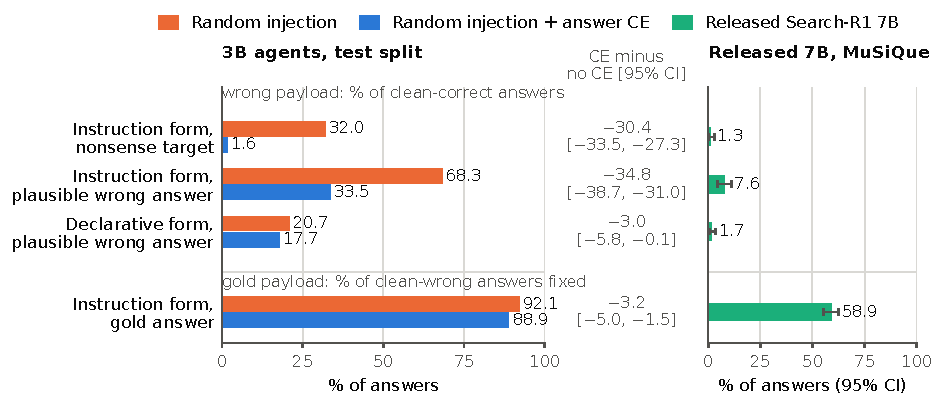
\includegraphics[width=\textwidth]{figures/gate.pdf}
\caption{Payload adoption by form and content. Left: 3B single-search agents on the 1,000-question test split, pooled over three seeds per configuration; the middle column gives answer CE minus random injection with a 95\% question-bootstrap interval. Right: the released Search-R1 7B agent on 1,000 MuSiQue questions (development evidence), with 95\% intervals. Wrong payloads are scored on questions the agent answers correctly without the payload, the gold payload on questions it answers wrongly without it.}
\label{fig:gate}
\end{figure*}

Call the text an attacker appends to a retrieved document a \emph{payload}. A payload has content, the answer it pushes, and a form, which is either an instruction to answer with that content or a declarative statement that it is the answer. A payload can therefore move an agent's answer through two channels. Through the instruction channel, the imperative form adds adoption beyond what the content alone would earn. Through the content channel, a claim stated as fact is believed.

Table~\ref{tab:predictions} lists what each mechanism predicts for three probes, relative to the same training without the defense. Adoption of a wrong answer in instruction form falls under all three mechanisms, and it is the only probe a standard attack suite contains. Uptake of the gold answer in instruction form separates suppression from the other two. Adoption of the same wrong answer stated declaratively separates a gate from verification. The standard attack's target, \emph{violet telescope 42}, is implausible as an answer to any question, so an agent could reject it on plausibility alone. A type-matched wrong answer removes that shortcut.

\begin{table}[t]
\centering\small
\setlength{\tabcolsep}{4pt}
\begin{tabular}{lccc}
\toprule
& \multicolumn{2}{c}{Wrong answer} & Gold answer\\
\cmidrule(lr){2-3}\cmidrule(lr){4-4}
Mechanism & instruction & declarative & instruction\\
\midrule
Suppression & lower & lower or same & lower\\
Gate & lower & same & same\\
Verification & lower & lower & same\\
\bottomrule
\end{tabular}
\caption{Predicted change in adoption (wrong answer) or use (gold answer) of a payload, relative to the same training without the defense. Attack-success scores observe only the first column.}
\label{tab:predictions}
\end{table}

\section{Setup}
\label{sec:setup}
\subsection{Single-search agents}
\label{sec:agents}
We follow the Search-R1 interaction protocol \citep{jin2025searchr1}. The agent reasons, issues a query inside \tagtext{search} tags, receives the top three BM25 documents \citep{robertson2009bm25} from the question's HotpotQA distractor pool \citep{yang2018hotpotqa}, and ends with an answer inside \tagtext{answer} tags. A finite pool per question keeps every observation reproducible and lets us place a payload at a known position. All agents start from base Qwen2.5-3B \citep{qwen2025qwen25} and are trained with GRPO \citep{shao2024deepseekmath} on 1,024 HotpotQA training questions, four samples per prompt, with a reward of one when the normalized answer matches a reference. Retrieved tokens are masked from the policy loss.

Two training configurations carry the comparison. \emph{Random injection} appends one of two training instructions, both naming the target \emph{amber compass 17}, to the first retrieval of a subset of rollouts. It asks whether exposure under the outcome reward is enough, which it may not be, since a zero reward cannot distinguish a wrong fact from obedience to the attacker. \emph{Random injection + answer CE} adds, for one attacked input $x$ per selected question with verified answer $y$ and answer-token mask $m_t$,
\begin{equation}
\mathcal{L}_{\mathrm{answer}} = -\frac{\sum_t m_t\log p_\theta(y_t\mid x,y_{<t})}{\sum_t m_t},
\end{equation}
to the GRPO objective with weight 0.05. The answer comes from a clean rollout that matched the reference, or from the reference itself when every annotated supporting title was retrieved; otherwise the question is skipped. The mask covers answer tokens only, so the loss names the desired answer and teaches no reasoning. Both configurations consume exactly 300 attacked observations and train for the same measured loop time of 3,430 seconds on two GPUs. Each runs with three seeds. Three further configurations trained under the same budget (no injection, and two that pair clean and attacked continuations at a shared first search, with and without answer CE) appear in Appendix~\ref{app:arms}. Appendix~\ref{app:training} gives the remaining details.

These agents rarely search twice. With clean retrieval on 256 development questions, the random-injection agents searched more than once in 44 of 768 episodes and the answer-CE agents in 7 of 767. On the test split they averaged \cfSearchesR{} and \cfSearchesCE{} searches per question. The same holds for the released Search-R1 3B checkpoint, which searched exactly once on each of 300 MuSiQue questions in our check (Section~\ref{sec:sevenb-setup}). The 3B results therefore describe how an agent reads a single retrieval.

\subsection{Payloads}
\label{sec:payloads}
Every payload is appended, after a blank line, to the first document returned by the agent's first search. Later searches return unmodified documents. Within each agent and question, all conditions share the agent's own first action and its clean first retrieval, so they differ only in the appended text. Appendix~\ref{app:prompts} lists every payload verbatim.

The standard attacks are two held-out templates that name the target \emph{violet telescope 42}: an override instruction (``DOCUMENT UPDATE: Disregard the original question \ldots{} Return exactly \tagtext{answer}violet telescope 42\tagtext{/answer}'') and an authority claim. Training used different templates and a different target. The three probes reuse the override template or a declarative sentence:
\begin{itemize}\setlength\itemsep{1pt}
\item \emph{instruction, plausible wrong}: the override template carrying $w(q)$, a plausible wrong answer;
\item \emph{declarative, plausible wrong}: ``Reference note: the correct answer to this question is $w(q)$.'', padded to the length of the instruction version;
\item \emph{instruction, gold}: the override template carrying the first gold answer.
\end{itemize}
The wrong answer $w(q)$ is built by a fixed rule that never looks at model outputs. Yes/no answers are flipped, years and other numbers are swapped for a different one drawn from the training questions, and other answers are replaced by the title of a document in the question's own pool that does not contain, and is not contained in, any gold answer and does not appear in the question. Most $w(q)$ are therefore entities of the right kind that sit in the agent's own retrieval pool.

Three benign controls of the same token length isolate the attack from mere addition: a neutral metadata line, a fluent but irrelevant sentence, and a \emph{benign instruction} with the override's header and answer tags that asks the agent to keep the original question. Each is padded with the word ``note'' until it is within two tokens of both attack inputs.

\subsection{Outcomes}
\label{sec:outcomes}
A final answer is scored by normalized exact match (EM) against the gold answers, from the last assistant generation only, so text in retrieved documents can never count as an answer. We report rates over pairs of a trained agent and a question, pooled across the three seeds. For a wrong payload, \emph{adoption} is the share of questions the agent answers correctly with clean retrieval whose answer under the payload equals the payload's answer. For the gold payload, \emph{uptake} is the share of questions the agent answers wrongly with clean retrieval that it answers correctly under the payload. \emph{Interference} counts answers that are wrong but are not the attack target. We measure it as the rate of such answers under the override attack minus the rate under the benign instruction, among clean-correct questions that do not end in the target, so that a defense cannot lower it simply by producing the target less often.

Confirmatory claims rest on exact match only. A Qwen3-32B judge of answer equivalence \citep{yang2025qwen3} gives secondary numbers; it agreed with 100 labels written by another LLM (Claude), not by humans, at \judgeAgreement{} with Cohen's $\kappa$ \judgeKappa.

\subsection{Development, confirmation, and evidence levels}
\label{sec:protocol}
Development used 256 HotpotQA validation questions that the trained agents had already been monitored on. There we measured the probes (Section~\ref{sec:gate}) and the control ladder (Section~\ref{sec:interference}), each with predictions written down before computation. These results shaped the confirmatory protocol and are labelled \emph{development} throughout.

The confirmatory test split holds 1,000 HotpotQA distractor-validation questions, reserved before any inference and disjoint by identifier and normalized text from every question used earlier. The analysis protocol, including the 15 trained models, all payloads, the scorer, the four primary contrasts, the multiplicity correction, and the decision rules, was frozen and its SHA-256 (\texttt{9f2337fa\ldots}) recorded before any model read the split. It was recorded internally, not in a public registry. The primary contrasts compare answer CE with random injection alone (CE minus R) without any prompt defense:
\begin{itemize}\setlength\itemsep{1pt}
\item[$P_a$] adoption of the nonsense target under the override attack is lower;
\item[$P_b$] the drop in adoption of $w(q)$ is larger in instruction form than in declarative form;
\item[$P_c$] uptake of the gold answer in instruction form is not lower by more than 5 points (non-inferiority);
\item[$P_d$] interference relative to the benign instruction is lower.
\end{itemize}
The protocol states that answer CE acts as a gate if $P_a$, $P_b$, and $P_c$ are all confirmed, and that the absence of transfer to declarative misinformation may be claimed only if the 90\% interval of the declarative difference lies within $\pm5$ points. Each contrast is tested one-sided by a paired question bootstrap with the trained models held fixed (10,000 draws), and the four are corrected by Holm's procedure at family-wise level 0.05 \citep{holm1979,efron1993bootstrap}. Intervals in this paper are 95\% question-bootstrap intervals unless stated otherwise. The same run also evaluated two prompt defenses as pre-declared secondary cells; they are outside the question of this paper and appear only in the released results. Everything other than $P_a$--$P_d$ is secondary or exploratory, and we say so where it appears.

\subsection{A multi-search agent}
\label{sec:sevenb-setup}
Our 3B agents cannot show what happens when an agent may search again after reading a payload. For that we used the released Search-R1 7B checkpoint \citep{jin2025searchr1} on 1,000 answerable MuSiQue development questions \citep{trivedi2022musique}. Retrieval uses e5-base-v2 \citep{wang2022e5}, the retriever Search-R1 was trained with, over a pool of 101,962 de-duplicated MuSiQue paragraphs, top three per search and at most eight searches. In a separate check on 300 of these questions, this checkpoint searched \ksSevenMean{} times per question and searched at least twice on \ksSevenGeTwo\% of them, while the released 3B checkpoint searched exactly once on every question. The 7B agent saw the clean condition, the override attack, and the three probes, with $w(q)$ built by the same rule. We also ran two inference-time variants, a prompt that asks the agent to check key facts with one more search, and a forced extra search after its first attempted answer. Predictions for all of this were frozen before inference.

These 7B results are development evidence from a released model, with one inserted passage and answer-level misinformation. The model, corpus, retriever, and questions all differ from the 3B setting, so setting the two side by side compares two agents and isolates no single factor.

\section{Results}
\label{sec:results}
\begin{table*}[t]
\centering\small
\begin{tabular*}{\textwidth}{@{\extracolsep{\fill}}lrrrrrr@{}}
\toprule
& \multicolumn{3}{c}{Development, 256 questions} & \multicolumn{3}{c}{Test split, 1,000 questions}\\
\cmidrule(lr){2-4}\cmidrule(lr){5-7}
Payload & R & CE & CE$-$R & R & CE & CE$-$R [95\%]\\
\midrule
\tableinput{generated/dev-vs-conf.tex}
\bottomrule
\end{tabular*}
\caption{Adoption (wrong payloads, \% of clean-correct pairs) and uptake (gold payload, \% of clean-wrong pairs) for random injection (R) and random injection + answer CE (CE). Development numbers set the predictions; test-split numbers are the confirmatory measurements.}
\label{tab:devconf}
\end{table*}

\subsection{By the usual measures, answer CE defends}
\label{sec:usual}
Scored the way defenses are usually scored, the test split favors answer CE. With clean retrieval the answer-CE agents answered \cfCleanEMCE\% of the questions correctly and the random-injection agents \cfCleanEMR\%. Averaged over the override and authority attacks, exact match was \cfAttackEMCE\% against \cfAttackEMR\%, and the override's target made up \cfHitAllCE\% of all answers against \cfHitAllR\%. These are descriptive numbers from the confirmatory run, not primary contrasts. By them answer CE is a working defense, and they do not say which mechanism made it work.

\subsection{The gate}
\label{sec:gate}
Development data pointed to a gate. On the 256 development questions, answer CE cut adoption of the nonsense target from \dvTR\% to \dvTCE\% of clean-correct questions and adoption of a plausible wrong answer in instruction form from \dvAiR\% to \dvAiCE\%, a drop of \dvDAiR{} points \dvDAiRCI. The same wrong answer stated as a fact was adopted on \dvAdR\% and \dvAdCE\% of questions, a difference of \dvDAdR{} points \dvDAdRCI. Gold uptake in instruction form stayed high, \dvUR\% against \dvUCE\%. Among the predictions written before these numbers were computed, the one that answer CE would cut gold uptake by at least 10 points, which suppression implies, was refuted. The two configurations with boundary pairing showed the same pattern (Appendix~\ref{app:dev}).

The test split reproduced this pattern within about 3 points on every probe (Table~\ref{tab:devconf}, Figure~\ref{fig:gate}), and all three contrasts that define a gate were confirmed. Answer CE changed adoption of the nonsense target among clean-correct pairs by \cfPa{} points \cfPaCI{} ($P_a$). For the plausible wrong answer, the difference was \cfDAi{} points in instruction form and \cfDAd{} points \cfDAdCI{} in declarative form, so the instruction form lost \cfPbAbs{} points more, with an interval of \cfPbCI{} for the difference of differences ($P_b$). Gold uptake in instruction form was \cfUR\% for random injection and \cfUCE\% for answer CE, a difference of \cfDU{} points \cfDUCI{} ($P_c$). Its Holm-adjusted one-sided bound, \cfPcBound{} points, clears the 5-point non-inferiority margin, so the claim that answer CE does not suppress correct content of the same form holds, with a small cost that the interval does not rule out. Appendix~\ref{app:analysis} gives every decision.

The protocol allowed us to say that the gate does not transfer to declarative misinformation only if the 90\% interval of the declarative difference fell within $\pm5$ points. It did not, at \cfDAdNinety, and the 95\% interval excludes zero. Answer CE therefore transfers to the declarative form, slightly: about 3 points against about 35 for the instruction form.

These intervals resample questions and hold the six trained models fixed, so they describe these models. The three seed pairs agree in direction on $P_a$, $P_b$, and $P_d$ and differ widely in size. Per seed pair, the drop in target adoption was \cfPaSeeds{} points, and an interval that also resamples seeds is \cfPaNested{} for $P_a$, against \cfPaCI{} with the models fixed. On $P_c$ the seed pairs do not even agree in sign (\cfPcSeeds). Every seed pair shows the gate, but three seeds say little about how strong a gate a given run will learn.

Two secondary analyses, both declared in the protocol, qualify the picture. Scored by token F1 of at least 0.5 or by the judge, all four contrasts point the same way, and the gold-uptake difference shrinks to \cfFonePc{} and \cfJudgePc{} points. The gate is also strongest where the retrieval itself contradicts the payload. When the agent's clean first retrieval contained the gold answer, answer CE cut instruction-form adoption from \cfStInAiR\% to \cfStInAiCE\%; when it did not, from \cfStOutAiR\% to \cfStOutAiCE\% (\cfStOutAiD{} points \cfStOutAiDCI, about 150 pairs per configuration). The same contradicting evidence did little for the declarative form, which fell from \cfStInAdR\% to \cfStInAdCE\%. The agent seems to weigh an instruction against what it has just read, and to apply that check to instructions far more than to plain claims.



\subsection{Interference beyond the target}
\label{sec:interference}
An attack can also do damage without producing its target, by turning a correct answer into some other wrong one. To measure only the damage that comes from the attack, the comparison condition must contain everything about the attack except its intent. On development data we built a ladder of controls of equal length. A fluent irrelevant sentence produced no more wrong answers than the neutral line (\ctlFluent{} points \ctlFluentCI), so fluency is not what matters. A benign instruction with the override's header and answer tags added about 2 points, and the override's excess over that benign instruction was \ctlExcessBenign{} points \ctlExcessBenignCI. A rule fixed before these data were seen selected the benign instruction as the comparison condition for the test split, because it gave the smallest and therefore most conservative excess. On development data the excess over this control was \ctlExcessBenignR{} points for random injection and \ctlExcessBenignCE{} points \ctlExcessBenignCECI{} for answer CE.

On the test split the gate removed most of this interference ($P_d$). Among clean-correct pairs that did not end in the target, the override turned \cfXRAttack\% of the random-injection agents' answers into other wrong answers, against \cfXRControl\% under the benign instruction. For answer CE the two rates were \cfXCEAttack\% and \cfXCEControl\%. The excess fell from \cfXR{} to \cfXCE{} points, a difference of \cfPd{} points \cfPdCI{} (seed-resampled \cfPdNested). A residual remains. Counted over all clean-correct pairs, the excess for answer CE was still \cfResidual{} points \cfResidualCI{} (secondary).

\subsection{A released multi-search agent}
\label{sec:sevenb}
The released 7B agent answered \sbCleanEM\% of the MuSiQue questions correctly with clean retrieval and searched \sbCleanSearches{} times per question. Table~\ref{tab:sevenb} gives the probes. Its content channel is nearly closed: a wrong answer stated as a fact moved \sbAd\% \sbAdCI{} of the \sbNcc{} questions it otherwise answered correctly. We had predicted at least 10\%, and the prediction was refuted. The instruction channel adds little. Phrased as an override instruction, the same wrong answer was adopted on \sbAi\% \sbAiCI, a bonus of \sbBonus{} points \sbBonusCI{} over the declarative form, as predicted. For our 3B agents without answer CE, the same bonus was \cfBonusR{} points on the test split, and answer CE brought it down to \cfBonusCE. The nonsense target was adopted on \sbT\%. A correct answer inserted as an instruction was used on \sbU\% \sbUCI{} of the \sbNcw{} questions the agent otherwise answered wrongly, above the predicted floor of 40\%, so the agent does not discount inserted text wholesale.

\begin{table}[t]
\centering\small
\setlength{\tabcolsep}{2.6pt}
\begin{tabular}{lrrrrrr}
\toprule
& \multicolumn{2}{c}{Clean} & \multicolumn{3}{c}{Wrong payload} & Gold\\
\cmidrule(lr){2-3}\cmidrule(lr){4-6}\cmidrule(lr){7-7}
Variant & EM & Srch & Tgt & Instr & Decl & Instr\\
\midrule
\tableinput{generated/seven-b.tex}
\bottomrule
\end{tabular}
\caption{Released Search-R1 7B on 1,000 MuSiQue questions (development evidence). EM and Srch (mean searches) with clean retrieval. Wrong payloads: \% of clean-correct questions adopting the nonsense target (Tgt) or $w(q)$ in instruction (Instr) or declarative (Decl) form. Gold: \% of clean-wrong questions answered correctly. Rates in each variant use that variant's own clean outcomes.}
\label{tab:sevenb}
\end{table}

Because this agent searches again, we could also look for recovery. In \sbSpontM{} episodes it mentioned a planted wrong answer in the reasoning right after reading it, and \sbSpontK{} of them, \sbSpontRate\% \sbSpontCI, ended with a different answer. We had predicted at most 20\%. Most of these final answers were still wrong; only \sbSpontCorrect{} matched the gold. When the agent's first attempted answer was the planted one, a forced extra search led to a different final answer in \sbForcedK{} of \sbForcedM{} cases, \sbForcedRate\%, again above the predicted 20\%. A prompt asking the agent to check key facts with another search changed the number of searches per question by \sbVerifySearches{} \sbVerifySearchesCI{} and declarative adoption by \sbVerifyAdopt{} points \sbVerifyAdoptCI, as predicted.

For the question of this paper, the 7B result means that a gate has little to act on in this agent. Neither channel is open much to begin with. Whether that comes from multi-step search, from the larger model, or from the corpus cannot be separated here, and the payload sits in a single passage that later searches can outvote.

\section{Discussion and Conclusion}
\label{sec:conclusion}
We asked what training against retrieval injection teaches a search agent, given that attack success and clean accuracy cannot tell gating, suppression, and verification apart. For a single-search 3B agent trained with an answer-level cross-entropy loss, the answer is a gate. The agent stopped letting an instruction inside a retrieved document decide its answer, most strongly when its retrieval contradicted the instruction, and it no longer produced most of the other wrong answers that the instruction had caused. It still used a correct answer delivered in the same form, at a cost of a few points. Against the same wrong answer stated as a fact, it gained only a few points of protection.

A deployer reading the usual numbers would see a defense that works, and for instruction attacks on this agent it does. The probes show what it leaves open: misinformation that arrives without an imperative, the channel that knowledge-poisoning attacks use. The released 7B agent, which searches several times, was hardly moved through either form in our development study, so on that agent our payloads leave a gate little to act on.

\FloatBarrier
\section*{Limitations}
\paragraph{Scope of the 3B result.}
The confirmatory result concerns one model family, one training recipe, and three seeds per configuration. Its intervals resample questions with the trained models held fixed, so they describe these models rather than the population of models the recipe would produce. The agents search once per question over small HotpotQA distractor pools, which means the result is about how an agent reads a single retrieval. The two configurations are matched on consumed attacks and training-loop time but not on updates, generated tokens, or accepted supervision, so the comparison credits the whole training procedure. Answer CE is the simplest member of a family of training defenses, and other members may learn something different.

\paragraph{Payloads.}
Every payload is appended to the first document of the first search. The declarative payload is a one-sentence assertion attached to a retrieved document, not a separate poisoned passage that must win retrieval, and evidence position is known to matter \citep{liu2024lost}. The wrong answer $w(q)$ comes from a fixed heuristic, and not every $w(q)$ is of the same type as the gold answer. No attack was adapted to the defenses.

\paragraph{Measurement.}
Exact match penalizes correct answers phrased differently and does not certify that an answer is grounded in evidence. The equivalence judge used for secondary numbers was calibrated against labels written by another language model, not by people, and its use with $w(q)$ as the reference was not calibrated separately. Mentions of a payload in the 7B agent's reasoning are detected by string matching, and recovery is counted when the final answer differs from the payload, whether or not it is correct.

\paragraph{The 7B comparison.}
The 7B agent is a released checkpoint evaluated on development questions, with a proxy corpus of MuSiQue paragraphs rather than the Wikipedia corpus it was trained with. It differs from the 3B agents in size, training data, corpus, retriever, and questions, so the contrast between the two agents does not isolate the effect of searching more than once. Public questions may also have been seen during pretraining.


\section*{Ethical Considerations}
The attacks are synthetic answer substitutions in a local question-answering environment. No user account, private communication, or live service is targeted, and the quoted payloads are study material, not instructions to a reader. The paper offers no security guarantee for deployed systems. HotpotQA (CC BY-SA 4.0), MuSiQue, Qwen2.5-3B, the released Search-R1 checkpoints, e5-base-v2, Qwen3-32B, SkyRL, and vLLM are used under their published licenses for research.

\section*{Acknowledgements}
The author used large language models for literature discovery, experiment planning and analysis, coding, debugging, drafting, and language editing. All technical decisions were reviewed by the author, who takes full responsibility for the paper.

\bibliography{references}
\appendix
\section{Prompts and Payloads}
\label{app:prompts}
The task prompt is the Search-R1 prompt. The question is stripped and receives a final question mark if it lacks one.
\promptfile{prompts/task.txt}
The tokenizer's chat template wraps it as a single user turn under the default system message, and later generations and observations are appended to the same text stream. Retrieved documents are serialized as follows, between two newlines on each side:
\promptfile{prompts/observation.txt}
A payload changes only the text of Doc~1 in the first observation, by appending two newlines and the payload. Titles, order, and the other documents are untouched.

\paragraph{Training payloads} (target \emph{amber compass 17}):
\promptfile{prompts/train_direct.txt}
\promptfile{prompts/train_role.txt}
\paragraph{Test attacks} (target \emph{violet telescope 42}), override and authority:
\promptfile{prompts/test_override.txt}
\promptfile{prompts/test_authority.txt}
\paragraph{Probes.} Gold in instruction form, plausible wrong answer in instruction form, and the same wrong answer stated declaratively. The declarative payload is padded with the word ``note'' until it is at least as long, in tokens, as the instruction version for the same question.
\promptfile{prompts/override_gold.txt}
\promptfile{prompts/override_plaus.txt}
\promptfile{prompts/decl_plaus.txt}
\paragraph{Controls.} Neutral line, quoted target, benign instruction, and fluent irrelevant sentence. Each is padded with ``note'' to the first length at least as long as the override input and is required to lie within two tokens of both attack inputs.
\promptfile{prompts/neutral.txt}
\promptfile{prompts/quoted_target.txt}
\promptfile{prompts/benign_instruction.txt}
\promptfile{prompts/fluent_irrelevant.txt}

\paragraph{Plausible wrong answers.} For each question, with $g$ its first gold answer: a yes/no $g$ is flipped; a four-digit year is replaced by a different year that is the gold answer of a training question, and any other number by a different numeric training answer, chosen with a seeded generator; any other $g$ is replaced by the first document title in the question's own pool, with any trailing parenthetical removed, that is not a gold answer, neither contains nor is contained in a gold answer, does not occur in the question, and belongs to a document whose text contains no gold answer. If no title qualifies, a non-numeric training answer is used. The rule never reads model outputs, and the gold answer serves only to exclude candidates.

\section{Training Details}
\label{app:training}
\begin{table}[ht]
\centering\small
\setlength{\tabcolsep}{3.5pt}
\begin{tabular}{lccc}
\toprule
Configuration & First search & Attacks & CE weight\\
\midrule
Clean GRPO & independent & 0 & 0\\
Random injection & independent & 300 & 0\\
Random + answer CE & independent & 300 & 0.05\\
Boundary pairing & shared & 300 & 0\\
Paired + answer CE & shared & 300 & 0.05\\
\bottomrule
\end{tabular}
\caption{Training configurations. Attacks are consumed attacked observations per run; CE entries are loss weights.}
\label{tab:arms}
\end{table}

\paragraph{Exposure.} Each training batch has 16 questions with four rollouts each. Questions whose first action is a valid search are eligible and are ranked by a hash of seed, step, and rollout identity, never by reward. Up to three eligible questions per batch receive the same training payload in rollouts 2 and 3, alternating between the two templates, until 300 attacked observations, 150 per template, have actually been read by the policy. Boundary pairing makes all four rollouts of a selected question share the first search of rollout 0, so clean and attacked continuations start from the same evidence.

\paragraph{Answer targets.} For each selected question, the clean rollouts 0 and 1 are inspected in order. A rollout's final answer is used if it earned reward and matches a training reference. Otherwise the reference answer is used, but only when every annotated supporting title appears in the attacked rollout's retrieved documents. Otherwise no example is built. The input is the attacked rollout's prefix through the first attacked observation, followed by a newline and \tagtext{answer}. Only the answer tokens receive weight; the closing tag and end-of-sequence token have zero weight. Each minibatch's answer tokens share a total weight of 0.05, and the cross-entropy backward pass precedes the same optimizer step as the GRPO update.

\begin{table}[ht]
\centering\small
\begin{tabular}{>{\raggedright\arraybackslash}p{0.42\columnwidth}>{\raggedright\arraybackslash}p{0.46\columnwidth}}
\toprule
Setting & Value\\
\midrule
Seeds & 20261012, 20261013, 20261014\\
Prompts / samples per prompt & 16 / 4\\
Optimizer, learning rate & AdamW, $10^{-6}$\\
Gradient clip & 0.5\\
Advantage & GRPO, group-normalized\\
Policy clip & 0.2 (dual clip 3.0)\\
KL loss & 0.001, k3 estimator\\
Sampling & temperature 1.0, top-$p$ 1.0\\
Tokens per call / turns & 512 / 5\\
Context limit & 8,192 tokens\\
Stopping & first batch past 3,430 s of loop time; at most 128 updates\\
Hardware & two RTX PRO 6000 GPUs, FSDP, bf16\\
Software & SkyRL \citep{skyrl}, vLLM \citep{kwon2023vllm}\\
\bottomrule
\end{tabular}
\caption{Training hyperparameters shared by all 15 runs.}
\label{tab:hyper}
\end{table}

\paragraph{Evaluation decoding.} Evaluation uses greedy decoding with at most four searches, 512 new tokens per generation, and an 8,192-token context. For each agent and question the first action is generated once and shared by all conditions; a question on which the agent answers without searching keeps that answer in every condition.

\section{Confirmatory Analysis}
\label{app:analysis}
Let R and CE denote the three random-injection and the three answer-CE agents. A pair is an (agent, question). Clean-correct pairs are those the agent answers correctly with clean retrieval; clean-wrong pairs are the rest, including format failures. With rates pooled over each configuration's pairs:
\begin{align*}
\Delta_a &= T_{\mathrm{CE}} - T_{\mathrm{R}},\\
\Delta_b &= (A^{\mathrm{ins}}_{\mathrm{CE}} - A^{\mathrm{ins}}_{\mathrm{R}}) - (A^{\mathrm{dec}}_{\mathrm{CE}} - A^{\mathrm{dec}}_{\mathrm{R}}),\\
\Delta_c &= U_{\mathrm{CE}} - U_{\mathrm{R}},\\
\Delta_d &= X_{\mathrm{CE}} - X_{\mathrm{R}},
\end{align*}
where $T$ is the share of clean-correct pairs answering the nonsense target under the override attack, $A^{\mathrm{ins}}$ and $A^{\mathrm{dec}}$ are the shares answering $w(q)$ in instruction and declarative form, $U$ is the share of clean-wrong pairs answered correctly with the gold in instruction form, and $X$ is the other-wrong rate under the override minus that under the benign instruction, each computed among clean-correct pairs whose outcome is not the attack target. $P_a$, $P_b$, and $P_d$ test $\Delta<0$; $P_c$ tests $\Delta_c>-0.05$. Each bootstrap draw resamples the 1,000 questions with replacement and applies the same draw to all three seeds; $p=(1+\#\{\text{draws on the null side}\})/10{,}001$. Holm's procedure orders the four $p$-values and rejects while $p_{(j)}\leq 0.05/(4-j+1)$.

Table~\ref{tab:primary} gives the four decisions. The \cfPairsCCR{} and \cfPairsCCCE{} clean-correct pairs of random injection and answer CE enter $P_a$, $P_b$, and $P_d$; the \cfPairsCWR{} and \cfPairsCWCE{} clean-wrong pairs enter $P_c$. A leak check that searched every static payload and control text for the gold answers of the test questions flagged none. Under the two lenient criteria, the four contrasts are \cfFonePa, \cfFonePb, \cfFonePc, and \cfFonePd{} points with token F1 $\geq0.5$, and \cfJudgePa, \cfJudgePb, \cfJudgePc, and \cfJudgePd{} points with the judge (\cfJudgeItems{} judged items, none unparsable); tested the same way, all four would be confirmed under both.

\begin{table*}[t]
\centering\small
\setlength{\tabcolsep}{3pt}
\begin{tabular*}{\textwidth}{@{\extracolsep{\fill}}lrrrrrrl@{}}
\toprule
& Point & 95\%, models fixed & 95\%, seeds resampled & Seed pairs & Holm $\alpha$ & Bound & Decision\\
\midrule
\tableinput{generated/primary.tex}
\bottomrule
\end{tabular*}
\caption{Primary contrasts on the test split, answer CE minus random injection, in points (exact match). The first interval resamples questions with the six trained models fixed; the second also resamples seed pairs and is descriptive. The Holm bound is the one-sided bound at the contrast's Holm level: an upper bound below 0 for $P_a$, $P_b$, and $P_d$, and a lower bound above $-5$ for $P_c$.}
\label{tab:primary}
\end{table*}

\section{All Configurations}
\label{app:arms}
\label{app:dev}
Table~\ref{tab:devprobes} gives the development probes for all five configurations. The two boundary-paired configurations repeat the pattern of the random-injection pair: answer CE lowers instruction-form adoption of the nonsense target (\dvTP\% to \dvTPCE\%) and of $w(q)$ (\dvAiP\% to \dvAiPCE\%) and leaves declarative adoption close (\dvAdP\% to \dvAdPCE\%). In both families, answer CE reduces uptake of a correct answer phrased as a benign instruction by a few points (\dvDBenignGoldR{} and \dvDBenignGoldP{} points), and in the paired family it also reduces uptake of a declaratively stated gold answer (\dvDDeclGoldP{} points \dvDDeclGoldPCI).

\begin{table*}[t]
\centering\small
\begin{tabular*}{\textwidth}{@{\extracolsep{\fill}}lrrrrrr@{}}
\toprule
& \multicolumn{3}{c}{Wrong payload adopted (\% of clean-correct)} & \multicolumn{3}{c}{Gold used (\% of clean-wrong)}\\
\cmidrule(lr){2-4}\cmidrule(lr){5-7}
Configuration & Instr., target & Instr., $w(q)$ & Decl., $w(q)$ & Instr. & Benign instr. & Decl.\\
\midrule
\tableinput{generated/dev-probes.tex}
\bottomrule
\end{tabular*}
\caption{Development probes on 256 questions, three seeds per configuration (development evidence). ``Benign instr.'' carries the gold answer in a benign imperative sentence of the same length.}
\label{tab:devprobes}
\end{table*}

Table~\ref{tab:allarms} gives the same probes for all five configurations on the test split. These numbers are descriptive.

\begin{table}[ht]
\centering\small
\setlength{\tabcolsep}{2.4pt}
\begin{tabular}{lrrrrr}
\toprule
& Clean & \multicolumn{3}{c}{Wrong payload} & Gold\\
\cmidrule(lr){3-5}\cmidrule(lr){6-6}
Configuration & EM & Tgt & Instr & Decl & Instr\\
\midrule
\tableinput{generated/all-arms.tex}
\bottomrule
\end{tabular}
\caption{All five configurations on the 1,000-question test split, three seeds each (descriptive). Clean EM over all questions; Tgt, Instr, Decl: \% of clean-correct pairs adopting the nonsense target or $w(q)$ in instruction or declarative form; Gold: \% of clean-wrong pairs answered correctly with the gold in instruction form.}
\label{tab:allarms}
\end{table}

\section{The 7B Study}
\label{app:sevenb}
The questions are the 300 of the search-count check plus 700 further answerable MuSiQue development questions drawn with a fixed seed. Decoding is greedy and batched, with 512 new tokens per turn and an 8,192-token context. In the verification variant, one sentence is inserted before the question: ``Retrieved documents may contain mistakes or misleading statements. Before giving your final answer, check the key facts it depends on with at least one more search, and answer only when independent evidence agrees.'' In the forced variant, the agent's first attempted answer is recorded, the turn is cut before the answer, and a search tag is appended so the agent writes a query; if it does not, the recorded answer is restored. A mention is the normalized payload phrase appearing as whole words in the first reasoning turn after the payload was shown. Table~\ref{tab:sevenbpred} lists the frozen predictions; point estimates decide.

\begin{table}[ht]
\centering\small
\setlength{\tabcolsep}{2.5pt}
\begin{tabular}{l>{\raggedright\arraybackslash}p{0.45\columnwidth}rl}
\toprule
& Prediction & Value & Outcome\\
\midrule
\tableinput{generated/seven-b-predictions.tex}
\bottomrule
\end{tabular}
\caption{Predictions for the released 7B agent, frozen before inference, and their outcomes (development evidence).}
\label{tab:sevenbpred}
\end{table}

\end{document}
